%%%%%%%%%%%%%%%%%%%%%%%%%%%%%%%%%%%%%%%%%
% Beamer Presentation
% LaTeX Template
% Version 1.0 (10/11/12)
%
% This template has been downloaded from:
% http://www.LaTeXTemplates.com
%
% License:
% CC BY-NC-SA 3.0 (http://creativecommons.org/licenses/by-nc-sa/3.0/)
%
%%%%%%%%%%%%%%%%%%%%%%%%%%%%%%%%%%%%%%%%%

%----------------------------------------------------------------------------------------
%	PACKAGES AND THEMES
%----------------------------------------------------------------------------------------

\documentclass{beamer}

\mode<presentation> {

% The Beamer class comes with a number of default slide themes
% which change the colors and layouts of slides. Below this is a list
% of all the themes, uncomment each in turn to see what they look like.

%\usetheme{default}
%\usetheme{AnnArbor}
%\usetheme{Antibes}
%\usetheme{Bergen}
%\usetheme{Berkeley}
%\usetheme{Berlin}
%\usetheme{Boadilla}
%\usetheme{CambridgeUS}
%\usetheme{Copenhagen}
%\usetheme{Darmstadt}
%\usetheme{Dresden}
%\usetheme{Frankfurt}
%\usetheme{Goettingen}
%\usetheme{Hannover}
%\usetheme{Ilmenau}
%\usetheme{JuanLesPins}
%\usetheme{Luebeck}
\usetheme{Madrid}
%\usetheme{Malmoe}
%\usetheme{Marburg}
%\usetheme{Montpellier}
%\usetheme{PaloAlto}
%\usetheme{Pittsburgh}
%\usetheme{Rochester}
%\usetheme{Singapore}
%\usetheme{Szeged}
%\usetheme{Warsaw}

% As well as themes, the Beamer class has a number of color themes
% for any slide theme. Uncomment each of these in turn to see how it
% changes the colors of your current slide theme.

%\usecolortheme{albatross}
%\usecolortheme{beaver}
%\usecolortheme{beetle}
%\usecolortheme{crane}
%\usecolortheme{dolphin}
%\usecolortheme{dove}
%\usecolortheme{fly}
%\usecolortheme{lily}
%\usecolortheme{orchid}
%\usecolortheme{rose}
%\usecolortheme{seagull}
%\usecolortheme{seahorse}
%\usecolortheme{whale}
%\usecolortheme{wolverine}

%\setbeamertemplate{footline} % To remove the footer line in all slides uncomment this line
%\setbeamertemplate{footline}[page number] % To replace the footer line in all slides with a simple slide count uncomment this line

%\setbeamertemplate{navigation symbols}{} % To remove the navigation symbols from the bottom of all slides uncomment this line
}

\usepackage{graphicx} % Allows including images
\usepackage{booktabs} % Allows the use of \toprule, \midrule and \bottomrule in tables
\graphicspath{ {../img/} }%setta il path predefinito per le immagini
\usepackage[utf8]{inputenc}
\usepackage{hyperref}

%----------------------------------------------------------------------------------------
%	TITLE PAGE
%----------------------------------------------------------------------------------------

\title[Trajectory Clustering survey]{Trajectory Clustering Alghorithms - Two scalable and Comovement-based approaches. } % The short title appears at the bottom of every slide, the full title is only on the title page

\author{Federico Naldini} % Your name
\institute[Università di Bologna] % Your institution as it will appear on the bottom of every slide, may be shorthand to save space
{
Alma Mater Studiorum - Università di Bologna, Cesena. \\ % Your institution for the title page
\medskip
\textit{federico.naldini3@studio.unibo.it} % Your email address
}
\date{15/10/2019} % Date, can be changed to a custom date

\begin{document}

\begin{frame}
\titlepage % Print the title page as the first slide
\end{frame}

%------------------------------------------------
\begin{frame}
\frametitle{Overview} % Table of contents slide, comment this block out to remove it
\tableofcontents % Throughout your presentation, if you choose to use \section{} and \subsection{} commands, these will automatically be printed on this slide as an overview of your presentation
\end{frame}
%------------------------------------------------
%----------------------------------------------------------------------------------------
%	PRESENTATION SLIDES
%----------------------------------------------------------------------------------------

%------------------------------------------------
\section{Comovement patterns} % Sections can be created in order to organize your presentation into discrete blocks, all sections and subsections are automatically printed in the table of contents as an overview of the talk

\begin{frame}

\frametitle{Che cosa sono i \textit{Comovements patterns}?}
I \textit{Comovements patterns} sono raggruppamenti di oggetti che hanno viaggiato assieme per un certo periodo di tempo.

L'interesse per questi insieme può essere basato su diversi fattori, come ad esempio il numero degli elementi, la durata del viaggio,
la loro effettiva vicinanza e il criterio utilizzato per calcolarla.

A seconda delle differenti caratteristiche utilizzate nel definire i raggruppamenti, è possibile definire delle tipologie di raggruppamenti.

\end{frame}
%------------------------------------------------

\begin{frame}

\frametitle{Tipologie di \textit{Co-movements pattern}}

Le tipologie di \textit{Co-movements pattern} possono essere divise sulla base di diversi fattori; 
tra tutti spicca in particolare la metrica di similarità utilizzata. 
Possono essere impiegate due misure:

\begin{itemize}

\item \textbf{Similarità basata sulla densità}

\item \textbf{Similarità basata sulla distanza}

\end{itemize}

\end{frame}

\begin{frame}

\frametitle{Similarità basata sulla densità}

\begin{itemize}

\item \textbf{Convoy}: Identifica raggruppamenti di oggetti che hanno percorso traiettorie simili per almeno \textit{T} istanti consecutivi, negli algoritmi classici prima viene applicato un algoritmo di \textit{clustering} basato sulla densità e successivamente viene effettuato \textit{pruning} sulla base del criterio temporale sopraespresso.

\item \textbf{Swarm}: Rispetto a \textbf{Convoy} scarta il vincolo di sequenzialità degli istanti temporali, basandosi solo sui vincoli spaziali.

\item \textbf{Platoon}:Rimuove il vincolo descritto da \textbf{Convoy}, sostituendolo con un vincolo locale sugli istanti consecutivi
tramite un parametro L che identifica la lunghezza 
minima di ogni sottosequenza di istanti consecutivi.

Inoltre aggiunge un altro parametro K, che identifica la lunghezza minima della sequenza temporale \textit{T} di ogni raggruppamento.

  

\end{itemize}

\end{frame}


\begin{frame}

\frametitle{Similarità basata sulla distanza}

\begin{itemize}

\item \textbf{Flock}: La stessa idea presentata in \textbf{Convoy}, ma utilizzando una metrica di similarità basata sulla definizione
di uno spazio chiamato \textit{disk} di raggio \textit{r}.


\item \textbf{Group}:Rilassa il vincolo temporale introdotto da \textbf{Flock} introducendo un vincolo sulla lunghezza delle sequenze di istanti consecutivi, analogamente a quanto fatto in \textit{Platoon}; tuttavia a differenza di quest'ultimo non introduce un vincolo sulla lunghezza totale della sequenza.


\end{itemize}

\end{frame}



%------------------------------------------------

\section{GCMP: un framework generico per il mining di Comovements}

\subsection{Obiettivi e definizione del problema e dei parametri}

\begin{frame}
\frametitle{General Co-movement Patter Mining}
Il framework \textbf{GCMP} si pone come obiettivo di mettere a disposizione degli utilizzatori una piattaforma configurabile per realizzare tutte le tipologie di \textit{Co-movement mining} sopradescritte.

In particolare definisce diversi parametri per la definizione del problema:
\end{frame}

\begin{frame}
\frametitle{General Co-movement Patter Mining: Parametri 1}

\begin{itemize}

\item \textbf{M}: Numero minimo di elementi presenti in un raggruppamento per considerarlo interessante.
\item \textbf{K}: Numero minimo di istanti temporali in cui un certo raggruppamento esiste.

\end{itemize}

\end{frame}

\begin{frame}
\frametitle{General Co-movement Patter Mining: Parametri 2}

\begin{itemize}

\item \textbf{L}: Data una sequenza temporale di istanti \textit{T}, si identificano \textit{z} sottosequenze tali che ogni sottosequenza è composta da istanti consecutivi(ad esempio con \textit{T} = (1,2,3,5,6) si ottengono due sottosequenze \textit{T'} = 
(1,2,3) e \textit{T''} = (5,6)); \textbf{L} identifica la lunghezza minima accettabile di tutte le \textit{z} sottosequenze così individuate(ad esempio con \textbf{L} = 3 la sequenza non rispetta il vincolo, mentre con \textbf{L} = 2 sì).

Una sequenza che rispetta il vincolo sopradescritto viene definita \textit{L-consecutive}
\item \textbf{G}:  Data una sequenza temporale di istanti \textit{T}, \textbf{G} identifica il massimo \textit{skew} accettabile tra un elemento della sequenza e il successivo. Una sequenza si definisce \textit{G-connected} se per ogni coppia di elementi consecutivi al suo interno 
lo \textit{skew} in questione è minore o uguale a \textbf{G} 

\end{itemize}

\end{frame}

\begin{frame}
\frametitle{General Co-movement Patter Mining: Definizione}

Un \textbf{GCPM} trova un set di oggetti \textit{O}, rimasti assieme per una sequenza di istanti \textit{T} che soddisfa i seguenti vincoli:

\begin{itemize}

\item \textit{Closeness}: per ogni istante di \textit{T}, gli oggetti \textit{O} devono appartenere allo stesso \textit{cluster}.
\item \textit{Significance}: La dimensione del raggruppamento deve essere maggiore di \textbf{M}.
\item \textit{Duration}: La dimensione di \textit{T} deve essere maggiore di \textbf{K}.
\item \textit{Consecutiveness}: \textit{T} è \textit{L-consecutive}.
\item \textit{Connection}: \textit{T} è \textit{G-connected}.


\end{itemize}

\end{frame}

\begin{frame}
\frametitle{General Co-movement Patter Mining: Parametri 3}

Configurando i vari parametri, posso ottenere le cinque tipologie di \textit{Co-movements}

\begin{center}
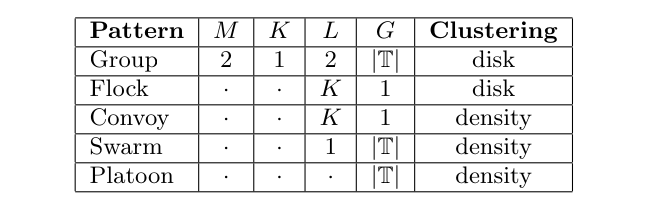
\includegraphics[scale=0.4]{ParametersConfiguration} 
\end{center}

\end{frame}



\subsection{Algoritmo di risoluzione}

\begin{frame}
	
	\frametitle{Overview}
	
	L'algoritmo di risoluzione proposto dal framework \textit{GCPM} si compone di tre fasi:
	
	\begin{itemize}
		
		\item \textbf{Generazione degli snapshot}
		
		\item \textbf{Star Partitioning}
		
		\item \textbf{Apriori Enumeration}
	\end{itemize}

Il risultato final dell'algoritmo consiste in una serie di tuple nella forma  \textless \textit{O,T}\textgreater,  dove \textit{O} è un insieme di oggetti identificati da un ID univoco, 
mentre \textit{T} rappresenta la sequenza temporale per cui l'insieme di oggetti \textit{O} ha viaggiato in luoghi vicini.
	
\end{frame}	

\begin{frame}
	\frametitle{Preprocessing dei dati}
	Unica operazione da eseguire per il preprocessing è l'unificazione di tutti i dati temporali alla stessa scala di misura:
	è importante che fra le misure temporali delle varie traiettorie sia definita una scala e dei criteri di misura che permettano di determinare se un istante è venuto o meno prima di un altro, 
	se due istanti sono consecutivi.
\end{frame}

\subsubsection{Generazione degli Snapshot}

\begin{frame}
	\frametitle{Generazione degli snapshot 1}
	Il primo passo dell'algoritmo consiste nella generazione degli \textit{Snapshots}, che altro non sono che raggruppamenti di oggetti in uno specifico istante temporale \textit{t}
	
\end{frame}

\begin{frame}
	\frametitle{Generazione degli snapshot 2}
	Ogni traiettoria associata ad un oggetto viene scomposta nell' insieme di punti che la compongono \textit{P}, ciascun punto \textit{p} viene poi aggregato in un nuovo insieme, chiamato \textit{P'} sulla base dell'attributo \textit{p.t}, ovvero la sua coordinata temporale.
	
	
\end{frame}

\begin{frame}
	\frametitle{Generazione degli snapshot 3}
	Su ogni \textit{P'} così individuato viene applicato un algoritmo di Clustering(\textit{DBSCAN}
	nel caso si necessiti di un algoritmo \textit{density based }, \textit{disk-based clustering} qualora si voglia utilizzare una metrica basata sulla distanza).
	I clustering di oggetti così individuati sono raggruppati in un set e vengono associati all'istante temporale \textit{t} che identifica \textit{P'}.
	
	Gli \textit{Snapshots} sono dunque nella forma \textless \textit{t, S(t)} \textgreater, dove \textit{t} è l'istante temporale mentre \textit{S(t)} è il set di clusters associato 
\end{frame}

\subsubsection{Star Partitioning}

\begin{frame}
	\frametitle{G \textsubscript{t} e G\textsubscript{A}}
Dato uno \textit{snapshot s\textsubscript{i}} definiamo il grafo \textit{G\textsubscript{ti}} come un grafo dove i nodi sono tutti gli oggetti del dataset e due nodi sono connessi da un arco se e solo se appartengono a uno stesso cluster.
Definiamo \textit{G\textsubscript{A}}, chiamato anche \textit{Associated Graph}, come l'insieme di tutti i \textit{G\textsubscript{i}} individuati dagli \textit{snapshot}:

L'insieme dei nodi sarà ancora una volta l'insieme degli oggetti e due nodi saranno connessi se compaiono all'interno di uno stesso cluster di un qualunque \textit{snapshot}.
Essendo possibile che due oggetti compaiano in più \textit{snapshot} all'interno di uno stesso cluster, sugli archi di questo grafo verrà mantenuta traccia degli istanti temporali in cui due oggetti compaiono nello stesso cluster. 
\end{frame}

\begin{frame}
	\frametitle{Directed star}
	\textit{G\textsubscript{A}} rappresenta il punto di partenza per catturare le relazioni tra coppie di oggetti, tuttavia non essendo  \textit{G\textsubscript{A}} un grafo orientato, occorre una tecnica per attraversare il grafo in maniera efficace e evitare di individuare coppie di nodi già visitate.
	
	\textbf{Directed Star} realizza tale struttura in due passi:
	\begin{enumerate}
		\item viene realizzato un ordinamento globale degli oggetti.
		\item si scorre \textit{G\textsubscript{A}} partendo dal nodo con Global ID=1, per ciascun nodo N si prendono in considerazione tutti i suoi vicini(ovvero connessi con un arco) con Global ID\textgreater   N.Global ID, vengono poi generate tutte le coppie 
		\textless \textit{N, V\textsubscript{i}: T(i)}\textgreater  dove \textit{N} è il nodo esaminato,
		\textit{V\textsubscript{i}} è l'i-esimo nodo vicino e \textit{T(i)} è la sequenza di istanti temporali contenuta nell'arco tra \textit{N} e \textit{V\textsubscript{i}}
	\end{enumerate}	
\end{frame}

\begin{frame}
	\frametitle{Ordinamento globale}
	Data la natura scalabile dell'algoritmo di generazione delle coppie sopracitato, è fondamentale che nel criterio di ordinamento e numerazione si scelga un criterio che permetta ad ogni nodo di avere circa lo stesso numero di vicini.
	
	Dati \textit{n} oggetti, ci sono \textit{n!} possibili ordinamenti.
	
	Utilizzare un criterio di ordinamento random, come ad esempio ordinando sugli IDs degli oggetti da performance tutto sommato accettabili.
\end{frame}

\subsubsection{Apriori Enumeration}

\begin{frame}
	\frametitle{Definizione di monotonicità}
	Dato un \textit{GCMP} con un objectset \{\textit{o\textsubscript{1}, ..., o\textsubscript{n}}\} , la fase di \textbf{Star Partitioning} produce coppie nella forma 
	\textless \textit{o\textsubscript{i}, o\textsubscript{j}. T} \textgreater.
	In linea teorica dovrebbe essere possibile applicare il principio \textit{Apriori} nella generazione dei candidati, tuttavia è facile dimostrare che la proprietà della monotonicità non vale per queste tuple.
\end{frame}

\begin{frame}
	\frametitle{Monotonicità classica}
Date due sequenze: 

	\textless \textit{o\textsubscript{i}, o\textsubscript{j}. 1,2,3,6} \textgreater
	
		\textless \textit{o\textsubscript{i}, o\textsubscript{z}. 1,2,3,7} \textgreater
		
		Con \textbf{L} = 2, \textbf{K} = 3 e \textbf{G} = 2
		
		E' intuitivo vedere che che entrambe le sequenze non risultano  \textit{L-Consecutive}.
		
		Al contrario, il superset ottenuto fondendo le due sequenze:
		
		\textless \textit{o\textsubscript{i},o\textsubscript{j}  ,o\textsubscript{z}. 1,2,3} \textgreater
		
		
		Risulta \textit{L-Consecutive}.
		
		E' quindi dimostrato che occorre trovare una nuova definizione di monotonicità.
		
\end{frame}

\begin{frame}
	\frametitle{Tre nuovi concetti}
	Per giungere a una nuova definizione di monotonicità serve introdurre tre nuovi concetti:
	
	\begin{itemize}
		\item \textbf{Maximal G-Connected sequence}
		\item \textbf{Decomposable sequence}
		\item \textbf{Sequence semplification}
	\end{itemize}
\end{frame}

\begin{frame}
	
	\frametitle{Maximal G-connected sequence}
	\textit{T'} è definibile come 
	\textit{MGS} di \textit{T} se \textit{T'} è sottosequenza di \textit{T} e non esiste \textit{T''} tale che \textit{T'} è sottosequenza di \textit{T''} e \textit{T''} è \textit{G-connected}.
	
	Ogni sequenza può avere \textit{n} MGS di dimensioni differenti.
	
	Ogni \textit{MGS} gode delle seguenti proprietà: 
	\begin{enumerate}
		\item Ogni \textit{MGS} è disgiunta dalle altre se non per un elemento in comune.
		\item Data una sequenza, l'unione di tutte le sue \textit{MGS} dà come risultato la sequenza stessa.
		\item Date due sequenze \textit{T\textsubscript{1}} e \textit{T\textsubscript{2}} dove
		\textit{T\textsubscript{1}} è sotto-sequenza di \textit{T\textsubscript{2}}, allora per ogni \textit{MGS} di \textit{T\textsubscript{1}} si può trovare una \textit{MGS} di 
		\textit{T\textsubscript{2}} tale che la \textit{MGS} di \textit{T\textsubscript{1}} sia sottosequenza della \textit{MGS} di \textit{T\textsubscript{2}}     
	\end{enumerate}
	
	\end{frame}


\begin{frame}
	\frametitle{Sequence simplification }
	Data una sequenza \textit{T}, questa viene definita come decomponibile se ogni sua \textit{MGS} è \textit{L-consecutive} e lunga almeno \textbf{K} elementi.
\end{frame}

\begin{frame}
	\frametitle{Decomposable sequence}
	Data una sequenza \textit{T}, viene prodotta una nuova sequenza \textit{T'} tramite una funzione \textit{Sim} che si compone di due passaggi: 
	\begin{enumerate}
		\item \textbf{f-step}: rimuove tutti i segmenti di \textit{T} che non sono \textit{L-consecutive}.
		\item \textbf{g-step} tra le \textit{MGS} ricavate dalla sequenza uscita dal passo precedente, rimuove quelle con dimensioni minori di \textbf{K}.
	\end{enumerate}
\end{frame}

\begin{frame}
	\frametitle{Nuova monotonicità}
   Dato un canditato \textit{C = \{O:T\}} dove \textit{O} è una sequenza di oggetti e \textit{T} una sequenza temporale, se \textit{Sim(T)} = $\emptyset$ allora il candidato può essere eliminato e così tutte le sue soprasequenze.
\end{frame}

\begin{frame}
	\frametitle{Algoritmo aPriori}
	\begin{enumerate}
		\item Ogni coppia va a generare il livello base della struttura
		\item Viene fatto pruning sulle coppie basandosi sulla funzione di semplificazione \textit{Sim}
		\item Tramite un indicatore di livello, vengono generati dei candidati di dimensione del livello, il join tra due candidati del livello precedente \textit{C\textsubscript{1}} e
		 \textit{C\textsubscript{2}} viene effettuato unendo gli object-set e intersecando le sequenze temporali.
		 \item Per ogni nuovo candidato viene calcolata la semplificazione e viene fatto pruning di conseguenza.
		 
		 Candidati che per uno dei vincoli parametrici non possono generare ulteriori candidati sono scartati
		 
		 \item Per migliorare le performance, si utilizza il principio della \textit{forward closure}: ogni pattern valido nei termini dei parametri espressi viene mandato in output.
	\end{enumerate}
\end{frame}

\begin{frame}
	\frametitle{Output}
	Un set di candidati nella seguente forma: 
	
	\begin{center}
		\huge  \textit{C = \{O:T\}} 
	\end{center}




	
	
\end{frame}

\begin{frame}
	\frametitle{Flow del framework}

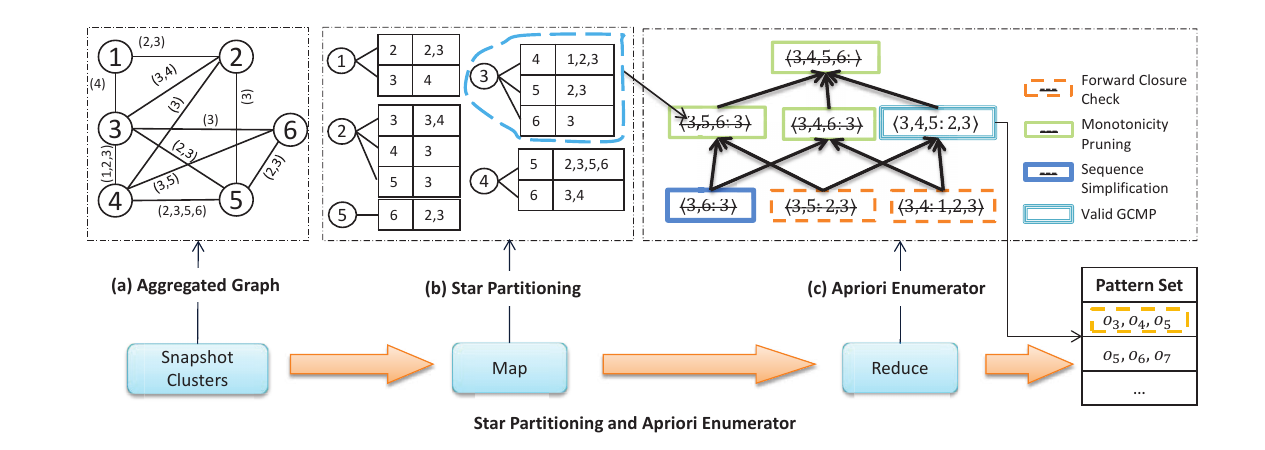
\includegraphics[scale=0.25]{GCMP-flow}
	
\end{frame}




\subsection{Subtrajectory Clustering}

\subsection{DSC Alghorithm}

\subsubsection{Subtrajectory Join}

\subsubsection{Trajectory Segmentation}

\subsubsection{Subtrajectory Clustering}




\begin{frame}
\titlepage % Print the title page as the last slide
\end{frame}

%----------------------------------------------------------------------------------------

\end{document}
